\paragraph{exponentiation}

ExponentiationGate is a gate for raising a value to a power. Trace table contains base, bits of the exponent, output, and intermediate value of the bits.

Take $A^{21} = A^{10101_b}$ for example to describe intermediate value, the bits are [1, 0, 1, 0, 1].

\begin{enumerate}
    \item Current bit = 1, we start from 1, and times $A^{bit}$ we get $A$
    \item Current bit = 0,
    \begin{itemize}
        \item Square prev\_intermediate\_value $A^{1_b << 1} = A^{10_b}$
        \item Then times $A^{bit}$ we get $A^{10_b} \times A^0 = A^{10_b}$
    \end{itemize}
    \item Current bit = 1,
    \begin{itemize}
        \item Square prev\_intermediate\_value $A^{10_b << 1} = A^{100_b}$
        \item Then times $A^{bit}$ we get $A^{100_b} \times A = A^{101_b}$
    \end{itemize}
    \item Current bit = 0,
    \begin{itemize}
        \item Square prev\_intermediate\_value $A^{101_b << 1} = A^{1010_b}$
        \item Then times $A^{bit}$ we get $A^{1010_b} \times 1 = A^{1010_b}$
    \end{itemize}
    \item Current bit = 1,
    \begin{itemize}
        \item Square prev\_intermediate\_value $A^{1010_b << 1} = A^{10100_b}$
        \item Then times $A^{bit}$ we get $A^{10100_b} \times A = A^{10101_b}$
    \end{itemize}
\end{enumerate}

And we get the last intermediate value $A^{10101_b}$ which should be equal to the output.

Let's take another example of a specific number $2^{13} = 2^{1101_b}$, and have a look at the trace cell:
\begin{center}
    \begin{tabular}{ |c|c|c|c|c|c|c|c|c|c| }
        \hline
        base & b\_0 & b\_1 & b\_2 & b\_3 & output & inter\_0 & inter\_1 & inter\_2 & inter\_3 \\
        \hline
        2 & 1 & 0 & 1 & 1 & 8192 & 2 & 8 & 64 & 8192 \\
        \hline
    \end{tabular}
\end{center}

The structure of gate is shown in \figref{fig:exponetiation-gate}.
\begin{figure}[!ht]
    \centering
    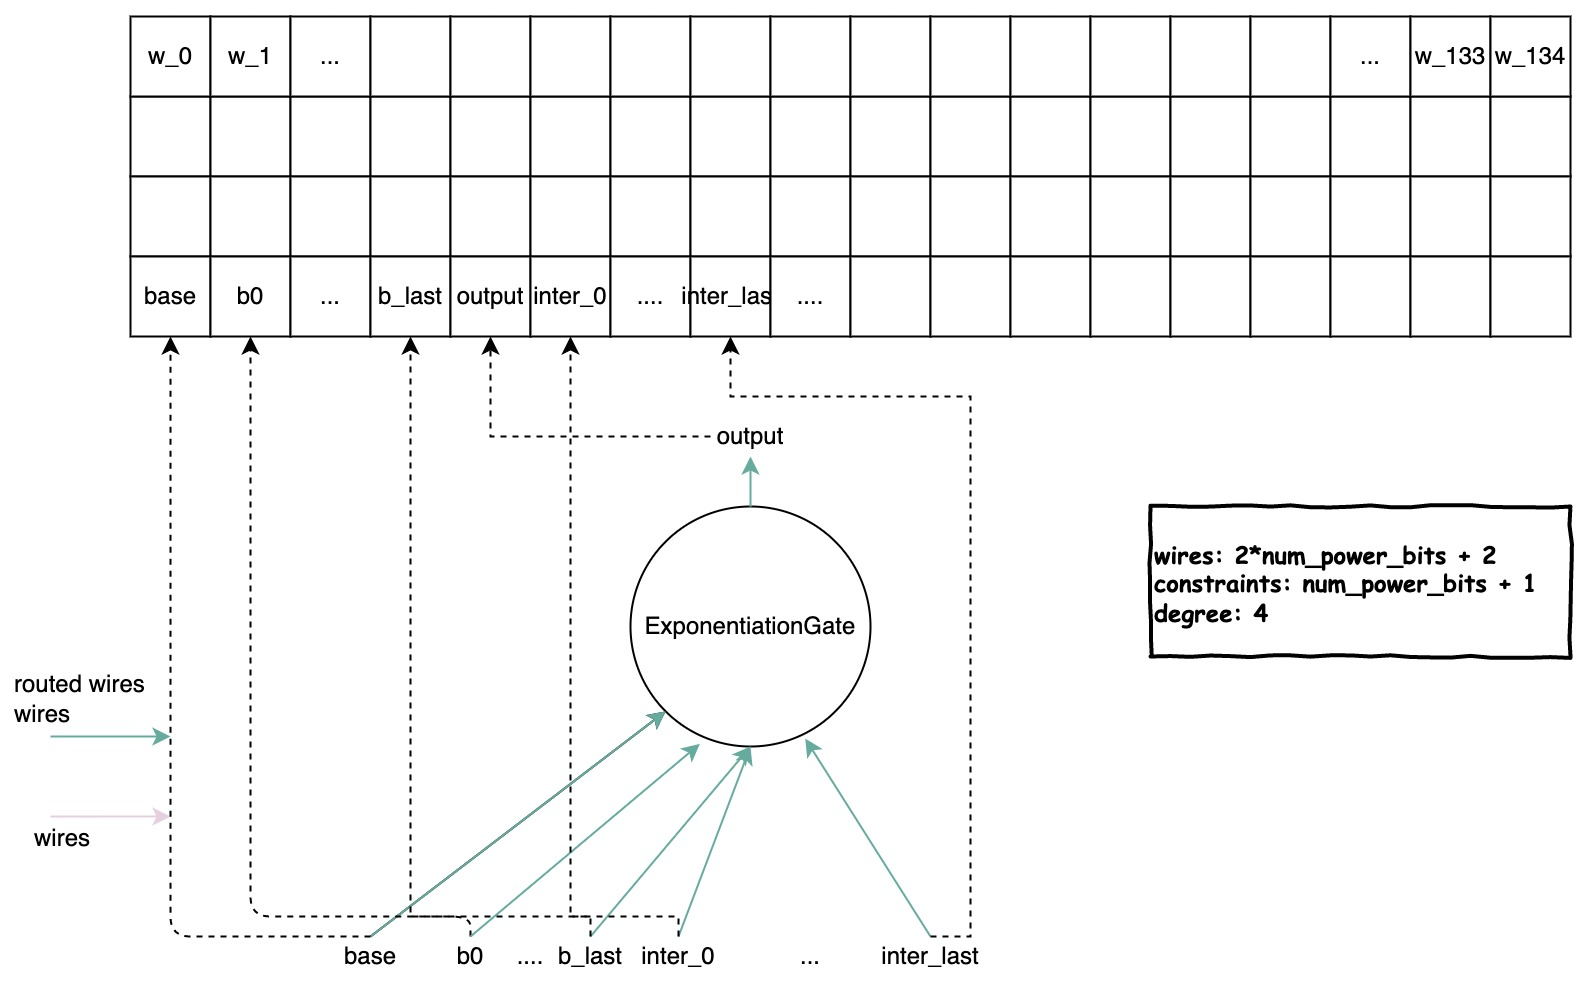
\includegraphics[width=0.5\textwidth]{gates/exponentiation.jpeg}
    \caption{ExponentiationGate}
    \label{fig:exponetiation-gate}
\end{figure}

Each step result constraint with intermediate values, and output is constrained with the final intermediated value, a total of $bits + 1$ constraints.
Degree of the gate is 4, which is determined by the intermediate calculation:
\begin{lstlisting}[language=rust]
let computed_intermediate_value =
            prev_intermediate_value * (cur_bit * base + not_cur_bit);
\end{lstlisting}
